\documentclass{article}
\usepackage[spanish]{babel}
\usepackage[utf8]{inputenc}
\usepackage[T1]{fontenc}
\usepackage{vmargin}
\usepackage{setspace}
\usepackage{enumerate}
\usepackage{graphicx}
\graphicspath{ {images/} }
\usepackage{float} 

\begin{document}
\begin{center}
\includegraphics[scale=0.3]{unison1.jpg}
\\
\vspace{0.5cm}
UNIVERSIDAD DE SONORA \\
\vspace{0.5cm}
DIVISIÓN DE CIENCIAS EXACTAS Y NATURALES \\
\vspace{0.5cm}
DEPARTAMENTO DE FÍSICA\\
\vspace{0.5cm}
LICENCIATURA EN FÍSICA\\
\vspace{0.5cm}
FÍSICA COMPUTACIONAL I
\vspace{2 cm}
\hrule
\vspace{1 cm}

{\huge \bfseries {Reporte de actividad 5}}
\\
\vspace{1 cm}
\hrule
\vspace{2 cm}
Ricardo Ruiz Hernández\\ 
\vspace{1 cm}
Profesor del curso\\
Dr. Carlos Lizárraga Celaya\\
\vspace{2 cm}
07 de marzo del 2018
\end{center}

\pagebreak
\begin{doublespace}


\hrule
\section{Introducción}
Esta práctica tuvo como principal objetivo que, de manera intensiva, como se menciona, aprendamos a manejar Emacs en la edición de archivos, con el claro objetivo de hacernos acreedores de la habilidad para limpiar datos, muy importante dentro de esta área del conocimiento.

\hrule

\begin{itemize}

\section{Conceptos}

\item CAPE: \textit{ES una herramienta que se utiliza para determinar en todo momento y lugar, cuan potenciales son los climas severos. Estas siglas corresponden a la cantidad de trabajo que hace un parcel en el ambiente} 
\item PW: \textit{Agua precipitable; expresa la cantidad de agua en términos de altura o masa.}

\section{Procesamiento y limpieza de los datos}

En el sitio de la universidad de Wyoming obtuve los datos de Smolensk, Rusia.
\item Se realizó un script, con el que se creó \textit{df2017}.
\item El siguiente paso fue filtrar los datos, mediante el comando \textit{grep}, solo dejamos los datos que contuvieran las palabras "CAPE", "PRECIP" y la fecha.\\
Es así que se creó un archivo al que se le llamó \textit{df2017\_PW.csv}
\item El archivo antes mencionado contenía palabras, o información que no nos sería útil, para lo que usamos Emacs. Así por medio de distintos comandos, limpiamos, quedándonos únicamente con lo numérico de lo que nos interesaba. 
\\
\begin{center}
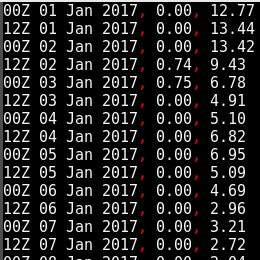
\includegraphics[scale=0.5]{act51.png}
\end{center}
Se utilizaros los siguiente comandos:
\\
\item Ctrl+w para borrar la parte seleccionada y mandarla a la memoria de igual manera.
\item Ctrl+y para recuperar la parte borrada.
\item Esc+<, esto nos lleva al inicio del documento.
\item Esc+\%, este comando abre el Query Replace, el cual hace que podamos remplezar un código por otro.
\item Seguidamente, volvemos a utilizar Ctrl+y para añadir lo que se mandó a la memoria en un principio, para después de un Enter, escribir su remplazo, en este caso, nada.
\item Se ejecutó este procedimiento las veces necesarias para obtener únicamente lo que requeríamos.

\item Se separó el archivo \textit{df2017\_PW.csv} en dos diferentes, correspondientes a 00Z y a 12Z; estos se llamaron \textit{df2017\_PW\_00Z.csv} y \textit{df2017\_PW\_12Z.csv}, respectivamente.
\begin{center}
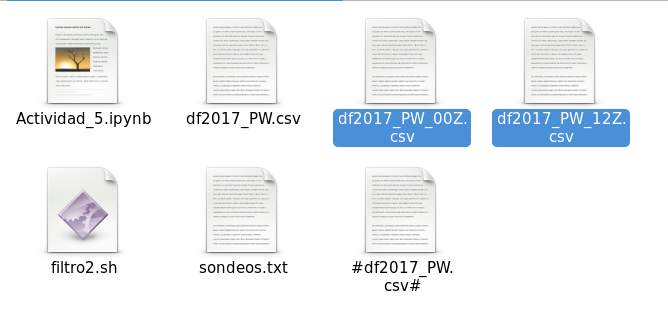
\includegraphics[scale=0.5]{act52.png}
\end{center}
\begin{center}
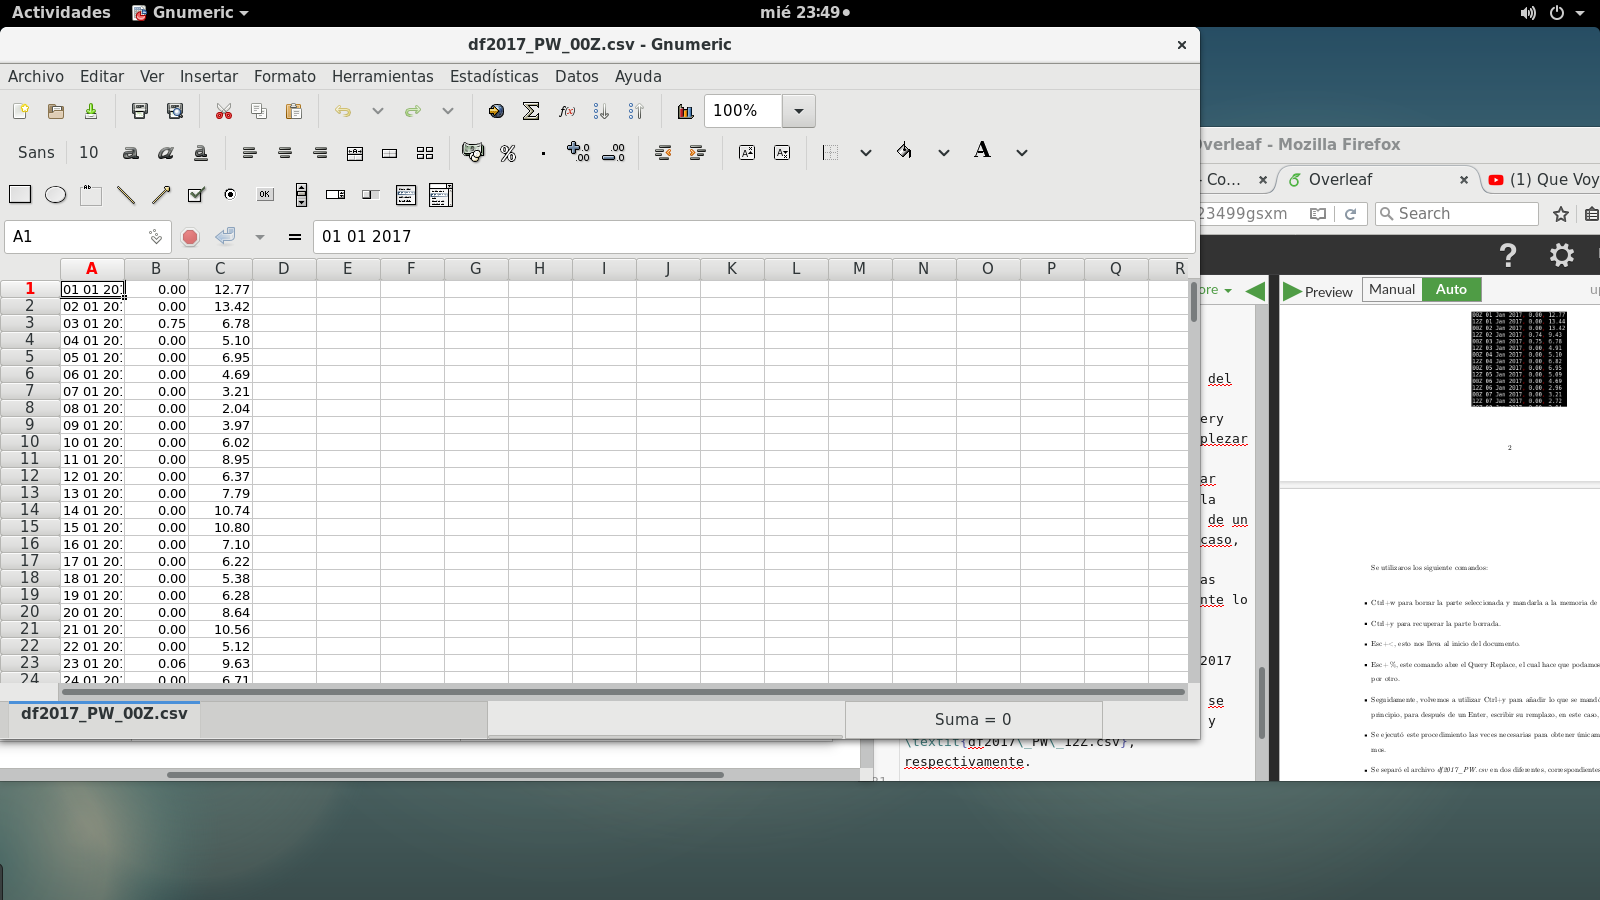
\includegraphics[scale=0.2]{act53.png}
\end{center}
\begin{center}
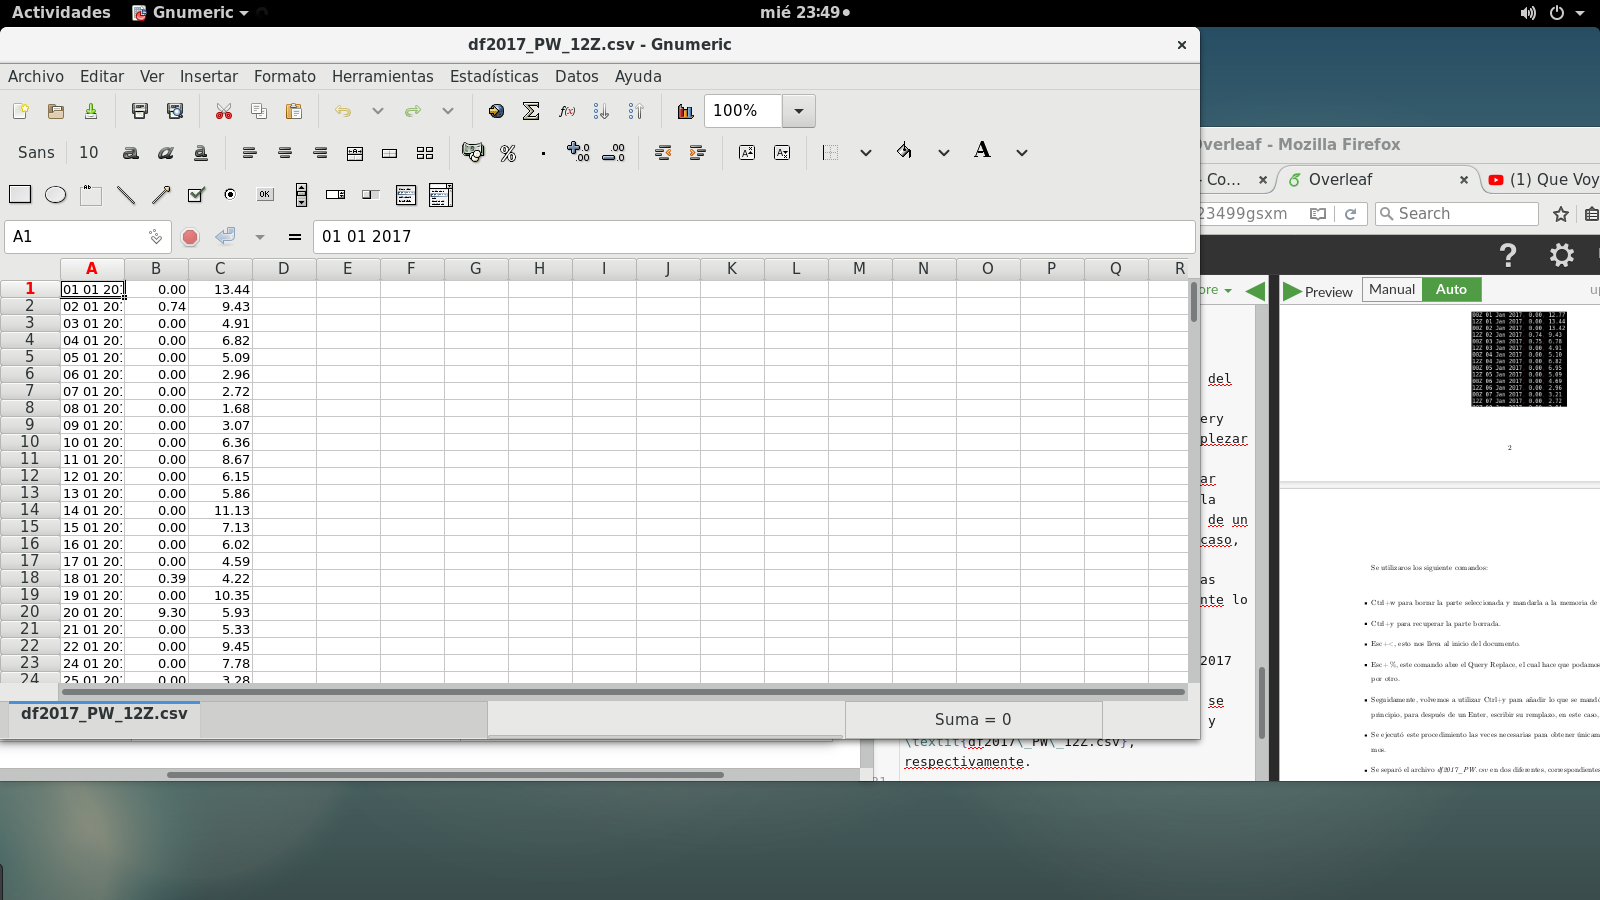
\includegraphics[scale=0.2]{act54.png}
\end{center}
\section{Análisis de datos}
Aquí le damos propósito a lo que hicimos anteriormente.
\item Después de cargar las bibliotecas, se leyeron los datos y se le asignó un formato a CAPE. Una vez esto, se creó una columna con formato de fecha, como se muestra a continuación.

\begin{center}
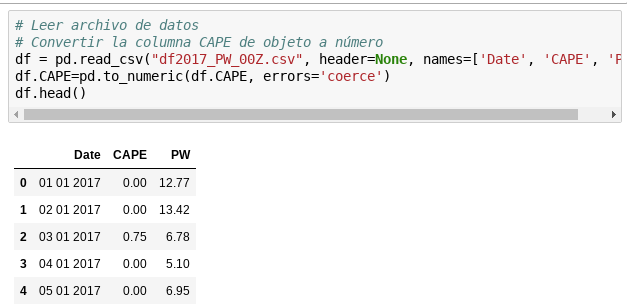
\includegraphics[scale=0.5]{act55.png}
\end{center}
\begin{center}
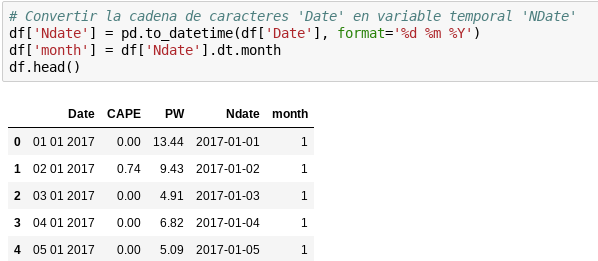
\includegraphics[scale=0.5]{act56.png}
\end{center}

\item Se cargaron las bibliotecas seaborn y matplotlib, estas fueron utilizadas para realizar gráficas tipo boxplot, además se compararon las variables (CAPE y PW).

\section{Resultados}
\item Gráficas tipo Boxplot de CAPE y PW, respectivamente: 
\\
\begin{center}
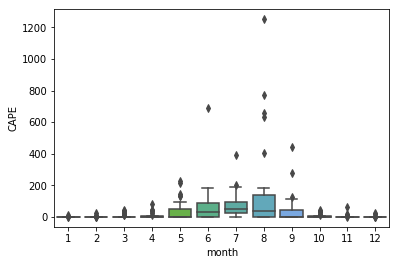
\includegraphics[scale=0.5]{act57.png}
\end{center}
\begin{center}
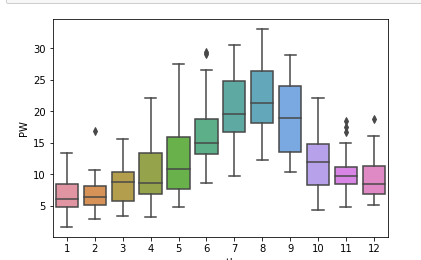
\includegraphics[scale=0.5]{act58.png}
\end{center}

\item En la gráfica de Jointplot se expone el coeficiente de correlación de Pearson:
\begin{center}
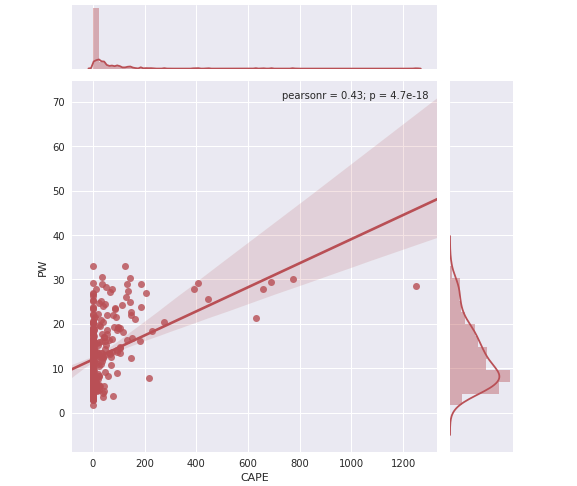
\includegraphics[scale=0.5]{act59.png}
\end{center}

\item En Lmplot se compara por cada mes, con el fin de ver como cambia con en cada estación del año:
\begin{center}
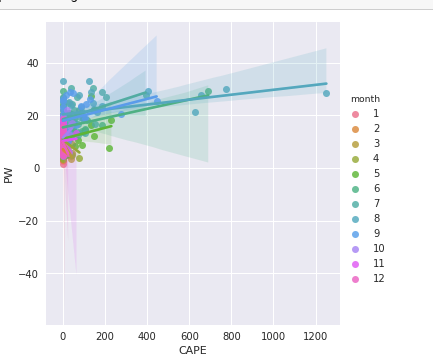
\includegraphics[scale=0.5]{act510.png}
\end{center}

\section{Conclusiones}
Mediante esta actividad pude percatarme de la importancia de saber limpiar datos, puesto que en muchas ocasiones, estos se encuentran con información de sobra o que no nos interesa en nuestra investigación. Además, aprendimos a cargar distintas bibliotecas para darle uso a estos datos.

\section{Bibliografía}
(2008) \textit{https://en.wikipedia.org/wiki/Precipitable\_water}

(2018) \textit{https://en.wikipedia.org/wiki/Convective\_available\_potential\_energy}

\section{Apéndice}
\begin{enumerate}
\item ¿Cómo se te hizo esta actividad? ¿Compleja, Difícil, Sencilla?
\\
\textit{No me pareció realmente compleja.}

\item ¿Qué te llamó más la atención? 
\\
Los comandos de Emacs, me pareció algo realmente útil e interesante.

\item ¿Qué parte fue la que menos te interesó hacer?
\\
Francamente, nada.
\item ¿Cómo mejorarías esta actividad? ¿Qué le faltó? ¿Qué sobró?
\\
Me pareció muy bien.

\item ¿Hasta este punto, qué te pareció el uso de Jupyter para programar en Python?
\\
Me ha parecido muy ameno, me gusta.

\end{enumerate}

\end{itemize}
\end{doublespace}
\end{document}
